\documentclass[11pt,a4paper]{article}
\usepackage[utf8]{inputenc}
\usepackage[T1]{fontenc}
\usepackage{lmodern}
\usepackage{textcomp}
\usepackage{amsmath,amssymb}
\usepackage{graphicx}
\usepackage{booktabs}
\usepackage{longtable}
\usepackage{array}
\usepackage{listings}
\usepackage{xcolor}
\usepackage[margin=1in]{geometry}
\usepackage{float}
\usepackage[hidelinks,breaklinks]{hyperref}
\usepackage{microtype}
\setlength{\parskip}{4pt}
\lstset{basicstyle=\ttfamily\scriptsize,breaklines=true,breakatwhitespace=false,
  postbreak=\mbox{\textcolor{gray}{$\hookrightarrow$}\space},frame=single,
  framerule=0.3pt,rulecolor=\color{gray!60},columns=fullflexible,keepspaces=true,
  showstringspaces=false,numbers=none,xleftmargin=4pt,xrightmargin=4pt,
  literate={\_}{{\_}}1}
\graphicspath{{figures/}}
\providecommand{\tightlist}{}
\title{Baryonic Feedback Bias in a DES-Y1-like 3x2pt Likelihood: Unmeasured Because the Pipeline Ignored Baryons}
\author{HEP-Genesis-Agent session record \\ \small Project: expert-baryon-lensing-bias-3}
\date{2026-10-24}
\begin{document}
\maketitle
\noindent\textit{\small This document is an AI-generated account of an interactive session with the HEP-Genesis agent. Its text was written by a language model strictly from the session record; figures and numbers come only from tool results obtained during the session. The supplementary material and the transcript, generated alongside, document exactly what ran. Verify independently before use.}
\vspace{1em}

\begin{abstract}
We set out to estimate how far cosmological parameters inferred from a DES/LSST-like weak-lensing (3x2pt) analysis would be biased if the analysis assumed gravity-only matter power while the true power followed a tabulated baryonic suppression $S(k)=P_{\rm hydro}/P_{\rm grav}$ from a HACC feedback emulator. That suppression is about 8\% at $k=3\,h\,\mathrm{Mpc}^{-1}$ and about 20\% at $k=8\,h\,\mathrm{Mpc}^{-1}$ at $z=0$. A firecrown likelihood was built on the offline DES-Y1-like test data vector: real space, 457 points, full covariance. Theory data vectors were then computed with no baryon correction and with a CCL Schneider15 baryon setting. The bias could not be measured. The firecrown pure-CCL mode used here ignores the cosmology's baryon switches, so both vectors are identical, with $\chi^2=551.57$ against the file's data in both cases. The tabulated $S(k)$ could not be injected either: there was no table interface, and the pyccl tool family was unavailable. A shear-only likelihood was rejected because of an inconsistent SACC file, and map simulations failed. Two pieces did work. A self-consistency check gave $\chi^2=0.00$ on a noiseless no-baryon realization. A one-parameter profile, with all other parameters fixed, gave a $\Delta\chi^2=1$ half-width of $\approx0.0099$ in $\sigma_8$ around $\sigma_8=0.81$. No baryon-induced $\Delta\chi^2$ or $\sigma_8/S_8$ shift was obtained.
\end{abstract}

\section{Introduction}
The user supplied two sets of ratio curves $S(k)=P_{\rm hydro}/P_{\rm grav}$ from a HACC baryonic-feedback hydrodynamics emulator. Both were linearly interpolated at $k=0.1,0.5,1,2,3,5,8\,h\,\mathrm{Mpc}^{-1}$ and $z=0,0.5,1$. The emulator's native grid has 799 points spanning $0.022$--$12.56\,h\,\mathrm{Mpc}^{-1}$.

The first set is a fiducial point: $\kappa_w=3.0$, $e_w=0.6$, $m_{\rm seed}=1.3$, $v_{\rm kin}=0.65$, $\epsilon_{\rm kin}=0.61$, $\omega_m=0.1375$, $\sigma_8=0.8$. It shows standard AGN suppression, for example $S(k=3)=0.915$ and $S(k=8)=0.803$ at $z=0$. The second is a weak-kinetic-feedback point with $v_{\rm kin}=0.1$ and $\epsilon_{\rm kin}=0.02$, which shows power enhancement ($S>1$) at intermediate to high $k$.

The question was how biased the inferred parameters of a DES/LSST-like cosmic-shear 3x2pt analysis would be if it assumed gravity-only power while the sky followed the fiducial suppression. The user asked for five steps:
\begin{enumerate}
\item build a representative DES-Y1-like firecrown likelihood with weak-lensing and photometric systematics (number counts not required);
\item inject the suppression via the CCL baryon mechanism, or explain why this is impossible and identify the closest knob, such as Schneider15 parameters approximating the $z=0$ suppression;
\item compute theory data vectors with and without baryons at the same fiducial point;
\item report the $\chi^2$ change and, if possible, the compensating $\sigma_8$ or $S_8$ shift, for instance from an augur Fisher matrix;
\item be explicit about approximations, failures, and uncertain numbers.
\end{enumerate}
The work consisted of a single assistant turn.

\section{Methods}
All computations used DESC tools on the \texttt{serve-desc.sh} server, with firecrown 1.16.0. The tool listings were consulted first. The \texttt{firecrown\_list\_examples} call listed four examples: \texttt{cosmic\_shear}, \texttt{cmb\_cross}, \texttt{sn\_srd} and \texttt{des\_y1\_3x2pt}, along with an offline test data vector \texttt{firecrown/tests/sacc\_data.hdf5}. The \texttt{ccl} tool family could not be imported (\texttt{No module named 'tools.ccl'}). The augur family (Fisher forecasts) was described but not run.

\paragraph{Likelihood.} \texttt{firecrown\_build\_likelihood} was run on the offline test SACC file. The result is a real-space experiment with 45 statistics and $n_{\rm data}=457$: $w(\theta)$ for lens0--4, $\gamma_t$, $\xi_+$ and $\xi_-$ over src0--3 and lens0--4. It requires 32 parameters, 11 cosmological and 21 nuisance. No scale cuts were applied.

The fiducial point is as follows.
\begin{itemize}
\item Cosmology: $\Omega_c=0.25$, $\Omega_b=0.05$ (so $\Omega_m=0.300$), $h=0.67$, $n_s=0.96$, $\sigma_8=0.81$, $\Omega_k=0$, $N_{\rm eff}=3.044$, $m_\nu=0$, $w_0=-1$, $w_a=0$, $T_{\rm CMB}=2.7255$.
\item Galaxy biases: 1.4, 1.6, 1.6, 1.9, 2.0 for lens0--4.
\item Lens photo-z shifts: 0.001, 0.002, 0.001, 0.003, 0.0.
\item Source photo-z shifts: $-0.001$, $-0.019$, $0.009$, $-0.018$.
\item Multiplicative shear biases: 0.012 in every source bin.
\item Intrinsic alignment: \texttt{ia\_bias}$=0.5$, \texttt{alphaz}$=0$.
\end{itemize}
The tool output states that halofit was used for the nonlinear power.

\paragraph{Shear-only attempt.} \texttt{sacc\_prepare\_for\_firecrown} kept only $\xi_\pm$. This produced a file with 227 points and a $227\times227$ full covariance (minimum diagonal element $2.38\times10^{-14}$). Building a likelihood on it failed, as described in Section~3.

\paragraph{Theory vectors.} \texttt{firecrown\_theory\_data\_vector} was called twice at the fiducial point. The first call set \texttt{baryons = none}. The second set \texttt{baryons = schneider15} with $\log_{10}M_c=14.095$, $\eta_b=0.213$ and $k_s=1000$. These Schneider15 values were chosen by the assistant without any fit to the emulator curve and were never evaluated.

\paragraph{Self-consistency and sensitivity.} The noiseless no-baryon realization was turned into a new likelihood. Its $\chi^2$ was then evaluated at the fiducial point (\texttt{firecrown\_compute\_loglike}). Next, $\sigma_8$ was profiled over 13 points in $[0.78,0.84]$ with all other parameters fixed (\texttt{firecrown\_scan\_loglike}).

\paragraph{Map simulations.} Two \texttt{namaster\_simulate\_maps} runs were attempted at $N_{\rm side}=64$, one with and one without Schneider15. Each used one shear tracer with $z_{\rm mean}=0.8$ and $z_\sigma=0.25$.

The full tool-call log is in the supplement.

\section{Results}
\subsection{Question 1: likelihood construction}
The full DES-Y1-like 3x2pt likelihood was built successfully (457 points). The shear-only variant was rejected by firecrown with the error ``Tracer lens0 does not have data points associated with it. Inconsistent SACC object.'' The preparation tool had dropped the $w(\theta)$ and $\gamma_t$ data but kept the lens tracers. None of the available tools could remove the lens tracers, so the analysis fell back to the full 3x2pt likelihood. This is broader than the user requested.

\subsection{Questions 2 and 3: injecting the suppression and computing theory vectors}
No tool accepted a tabulated $S(k,z)$. The pyccl family was not importable, so CCL could not be used directly to apply the table or to fit Schneider15 parameters to it.

The no-baryon theory vector is shown in Figure~\ref{fig:6}. It gives $\chi^2=551.57$ (log-likelihood $-275.785$) against the test file's data at the fiducial point.


\begin{figure}[H]
\centering
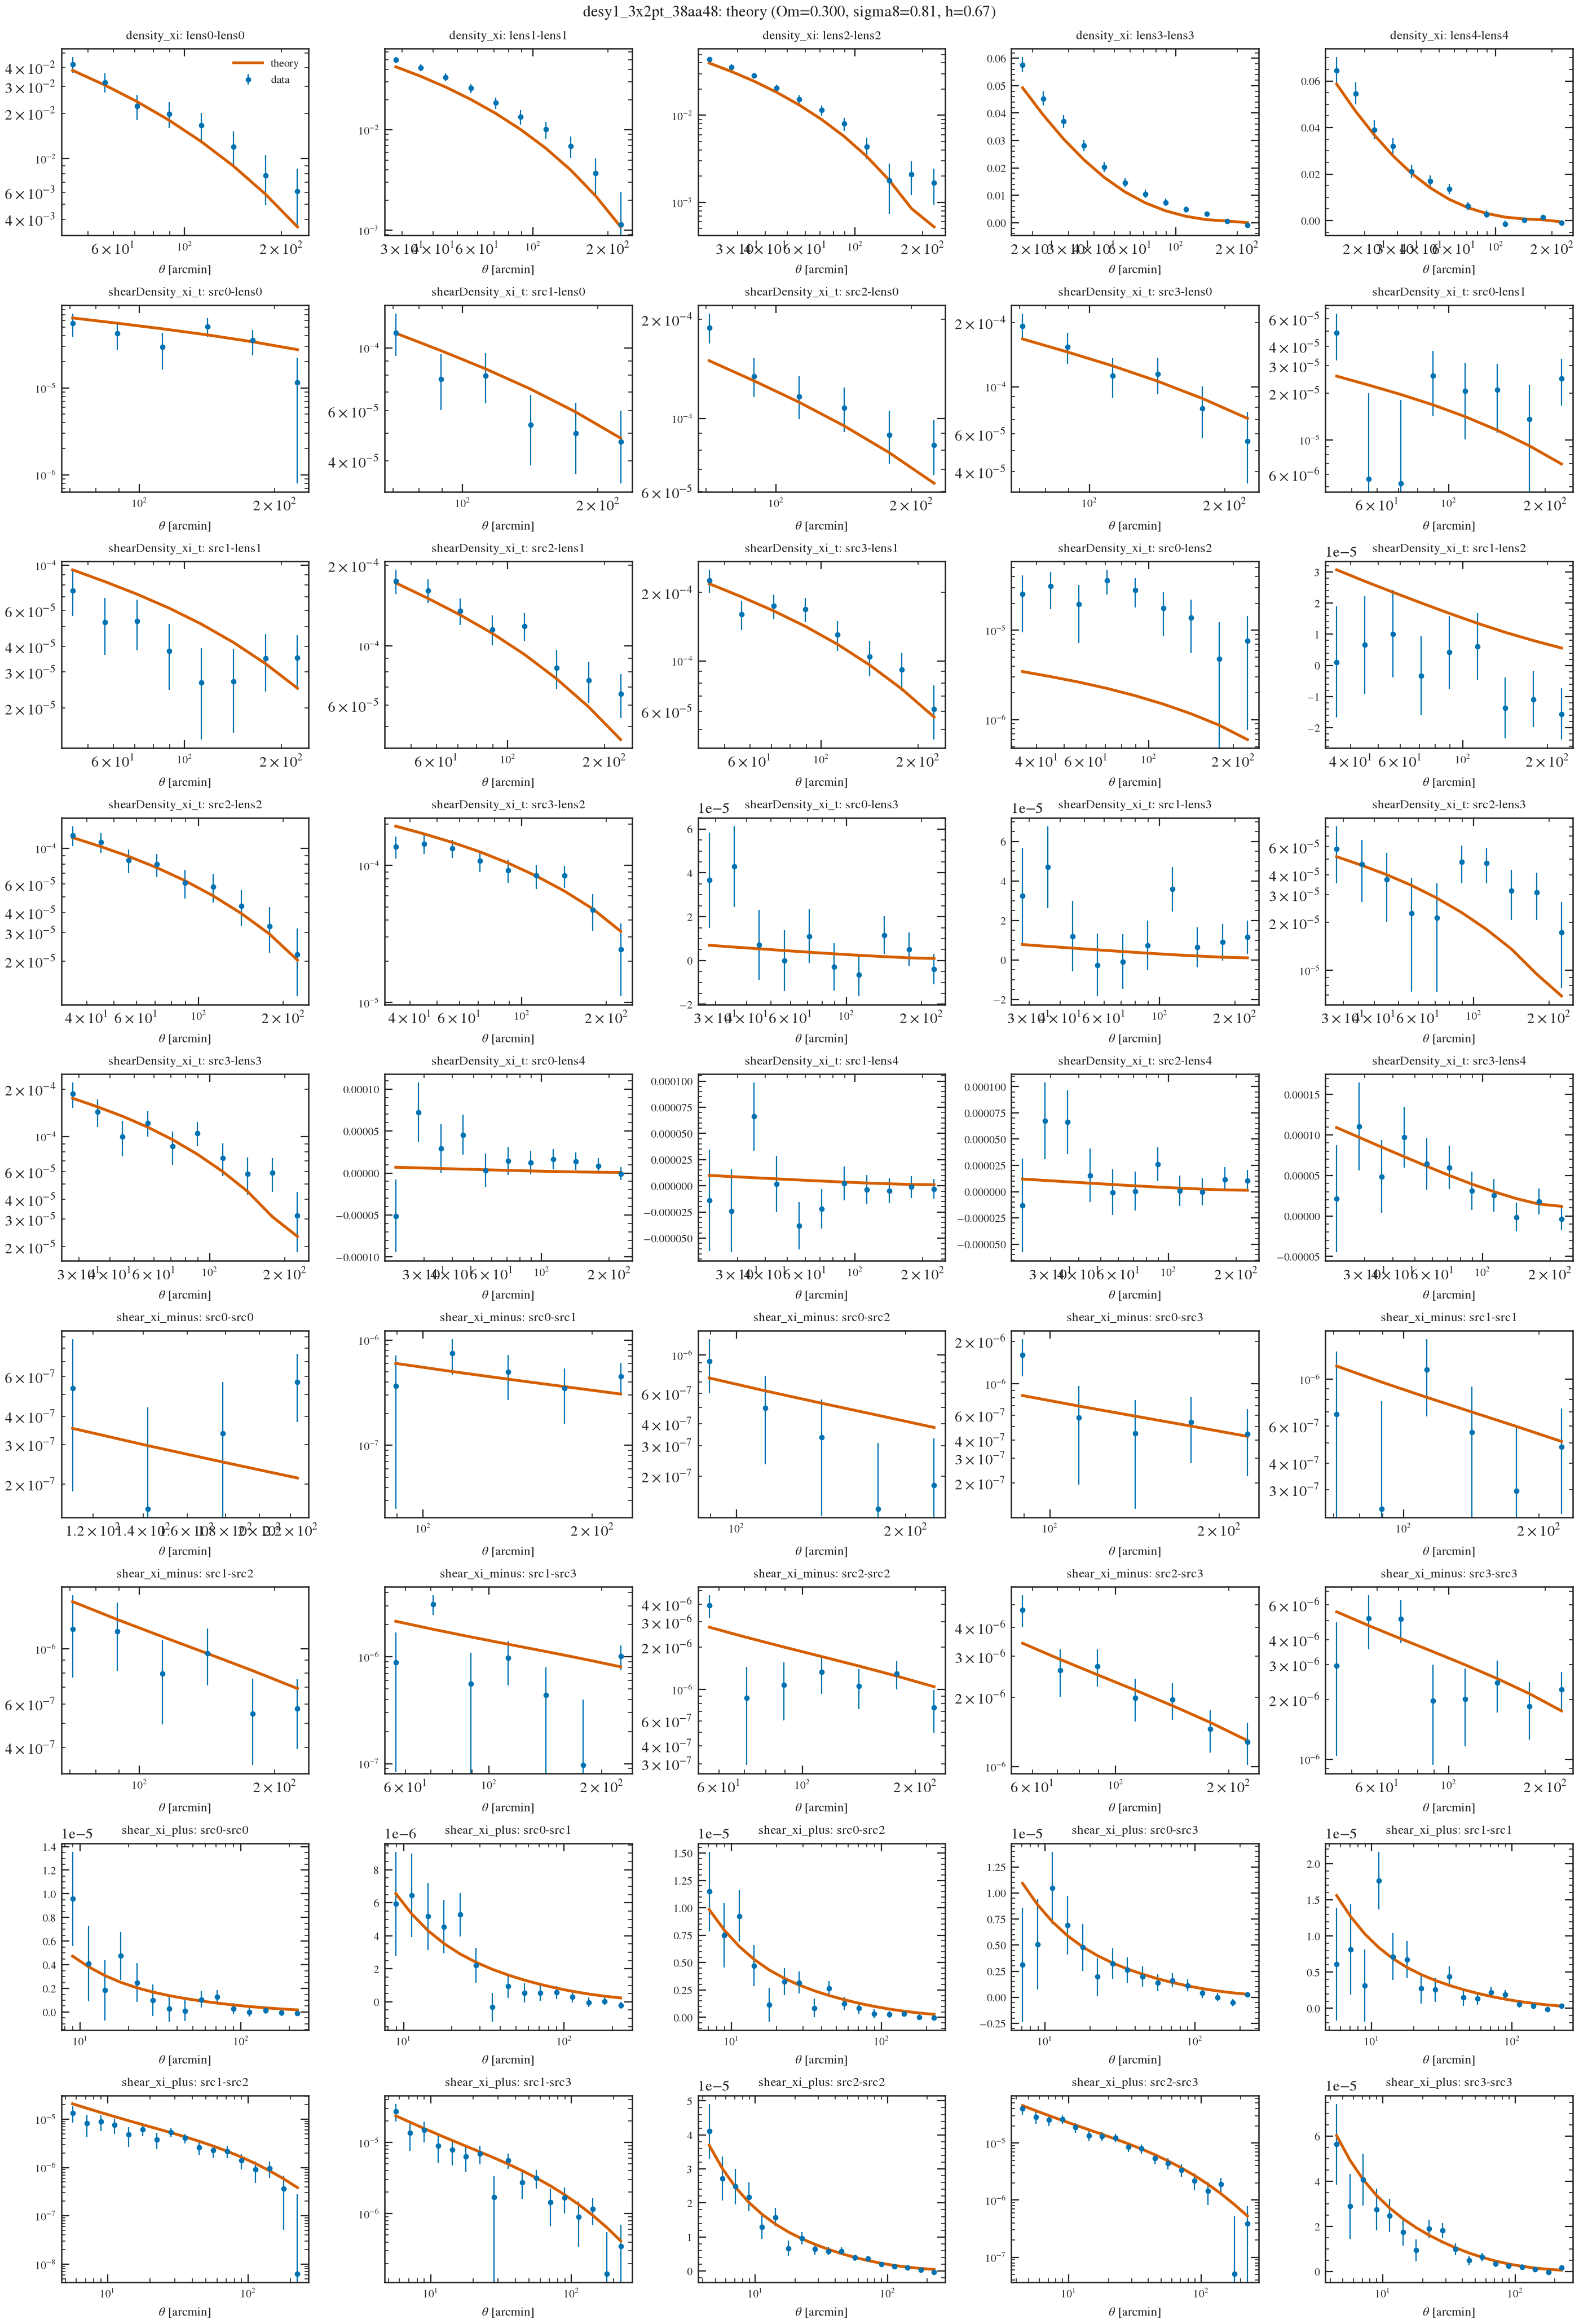
\includegraphics[width=0.85\textwidth,height=0.6\textheight,keepaspectratio]{fig-6.png}
\caption{theory\_vector\_912d53.png Produced in this session by \texttt{firecrown\_theory\_data\_vector} on \textit{serve-desc.sh}.}
\label{fig:6}
\end{figure}



The Schneider15 call returned the same $\chi^2=551.57$, with an identical log-likelihood. It also issued the warning: ``firecrown (pure-CCL mode) uses halofit without baryons/MG here; the cosmology's matter\_power\_spectrum/baryons/MG switches are ignored.'' The ``with baryons'' vector is therefore identical to the no-baryon one and carries no baryonic information.

Consequently, it remains unknown whether the chosen Schneider15 parameters reproduce the target 8\% suppression at $k=3\,h\,\mathrm{Mpc}^{-1}$ and 20\% at $k=8\,h\,\mathrm{Mpc}^{-1}$. They must be regarded as uncalibrated.

Map simulations were attempted as an alternative route. Both runs failed with ``Buffer has wrong number of dimensions (expected 1, got 2)''.

The assistant also made two qualitative points about the user's input curves; these are not tool results.
\begin{itemize}
\item It stated that Schneider15 has no redshift dependence. It would then be unable to follow the fiducial $S(k)$. At $k=8$, that curve weakens from $0.803$ at $z=0$ to $0.969$ at $z=1$. At $z=1$ it also turns back up, from $0.944$ at $k=5$ to $0.969$ at $k=8$.
\item It stated that Schneider15 cannot represent the $S>1$ enhancement of the weak-kinetic point, which has, for example, $S(k=3)=1.0165$ at $z=0$.
\end{itemize}

\subsection{Question 4: $\chi^2$ change and parameter shift}
The baryon-induced $\Delta\chi^2$ is zero only because the baryon setting was ignored. It is not a physical result. No compensating $\sigma_8$ or $S_8$ shift could be computed, and no augur Fisher matrix was run, since the assistant reported that augur also offers no baryonic $P(k)$.

Two auxiliary results were obtained. First, the likelihood rebuilt on the noiseless no-baryon realization gives $\chi^2=0.00$ at the fiducial point in every statistic, so the pipeline recovers its own input.

Second, Figure~\ref{fig:14} shows the $\chi^2$ profile in $\sigma_8$ with all other parameters fixed. The profile is close to parabolic, with $\chi^2=1.001$ at $\sigma_8=0.80$ and $1.030$ at $0.82$. At the ends of the scan it reaches $8.75$ at $0.78$ and $9.54$ at $0.84$. The parabolic fit gives $\sigma_8=0.81\pm0.00992$, and the $1\sigma$ interval is $[0.800,0.8198]$.


\begin{figure}[H]
\centering
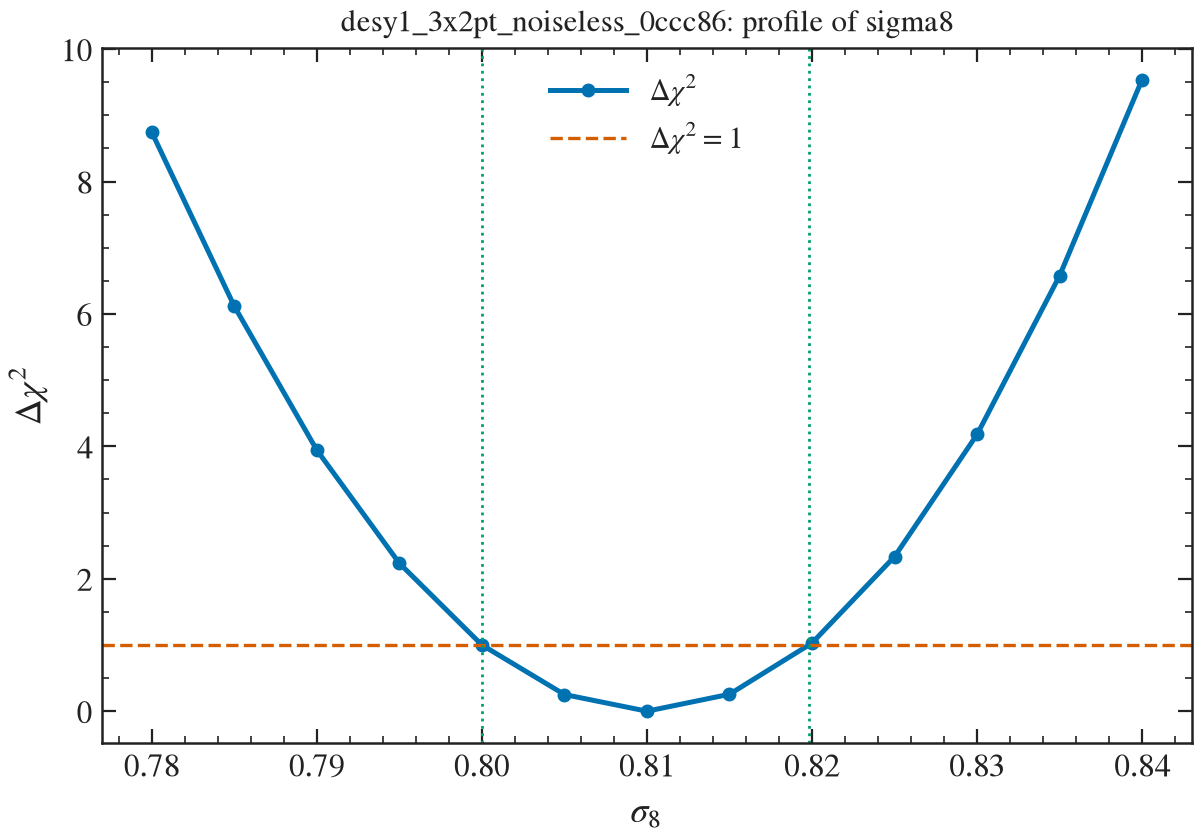
\includegraphics[width=0.85\textwidth,height=0.6\textheight,keepaspectratio]{fig-14.png}
\caption{scan\_sigma8\_63cd84.png Produced in this session by \texttt{firecrown\_scan\_loglike} on \textit{serve-desc.sh}.}
\label{fig:14}
\end{figure}



This width sets the scale against which a baryon-induced $\sigma_8$ shift would be judged. It is a conditional, unmarginalised width, computed with the DES-Y1 covariance and without scale cuts.

\section{Discussion}
The central failure is structural. The firecrown pure-CCL mode served here fixes the nonlinear power to halofit and silently drops the baryon and modified-gravity switches. Neither the CCL Schneider15 route nor the user's tabulated $S(k)$ could therefore reach the theory prediction.

The assistant noted that firecrown has a \texttt{pk\_modifier} example type, but the likelihood builder on this server does not expose it. A direct pyccl path, applying $S(k,z)$ to $P(k,z)$ and recomputing $\xi_\pm$, was likewise unavailable.

The assistant offered a rule-of-thumb estimate, which is its own reasoning and not a tool result. Since $\xi_+\propto\sigma_8^2$ roughly, a uniform fractional amplitude drop $\epsilon$ would lower the inferred $\sigma_8$ by about $\epsilon/2$. The real suppression is scale- and redshift-dependent, so the assistant expected it to project also onto $\Omega_m$, the intrinsic-alignment amplitude and the shear calibration. This estimate was not quantified.

The $\sigma_8$ width of $\approx0.01$ has two limitations: it is conditional on fixed nuisance and cosmological parameters, and it was obtained without the small-scale cuts a DES-like analysis would use. A realistic marginalised bias could differ substantially.

\section{Conclusions}
The session established a working DES-Y1-like 3x2pt firecrown likelihood (457 points). The pipeline is self-consistent ($\chi^2=0.00$ on its own noiseless output). The conditional $\sigma_8$ sensitivity is $\Delta\chi^2=1$ at $\pm0.0099$ around $0.81$.

The session did not measure any baryonic bias. The Schneider15 setting was ignored, giving identical data vectors ($\chi^2=551.57$ in both cases). The tabulated $S(k)$ could not be injected, the Schneider15 parameters were never calibrated, the shear-only likelihood and the map simulations failed, and no Fisher forecast was run.

The assistant identified these next steps:
\begin{enumerate}
\item Obtain a firecrown setup that applies an $S(k,z)$ correction, via \texttt{pk\_modifier}, or a pyccl environment in which the table can be applied to $P(k,z)$.
\item Build the likelihood on the suppressed data vector, evaluate the no-baryon model's $\chi^2$, and profile $\sigma_8$. A chain over $\Omega_c$ and $\sigma_8$ with nuisance parameters free would give the $S_8$ shift.
\item Apply standard small-scale cuts on $\xi_\pm$.
\end{enumerate}

\section*{Data and code availability}
All outputs of this session are collected in the project folder \href{file:///Users/nramachandra/hep-genesis-testing/projects/expert-baryon-lensing-bias-3}{\texttt{/\allowbreak{}Users/\allowbreak{}nramachandra/\allowbreak{}hep-genesis-testing/\allowbreak{}projects/\allowbreak{}expert-baryon-lensing-bias-3}}.
The session produced 11 data files; the supplement lists them.
Full documentation of how these results were obtained is in the supplementary material (\texttt{supplement.pdf}: implementation details, the tool-call log, the research board with every finding and its evidence, figures not shown here, and the code index) and the verbatim transcript (\texttt{transcript.pdf}), generated alongside this report.


\end{document}
